\chapter{Corrosion and Protection}\label{ch:b2:corrosion}

Leave a drop of salt water on a clean piece of steel. After a day the metal is
pitted at the centre of the drop, while the rust has formed in a ring near its
edge, where the oxygen of the air dissolves. The iron dissolves where there is
the least oxygen, and the oxygen is reduced where there is the most: the drop
is a cell that nobody built, short-circuited through the metal itself. This
chapter reads corrosion on \omterm{def:b2:current-potential-curves:ie-curve}{current--potential curves}, explains why a
scratched galvanised sheet does not rust while a scratched tin can does, and
designs the protection of a buried pipeline.

\begin{recall}
The Year 1 volume: E--pH diagrams of metals and their domains of immunity,
corrosion and \omterm{def:b2:corrosion:passivation}{passivation} (``whether a coat protects is a kinetic matter'').
\Cref{ch:b2:current-potential-curves}: \omterm{def:b2:current-potential-curves:ie-curve}{current--potential curves}, \omterm{def:b2:current-potential-curves:limiting-current}{limiting
currents}. \Cref{ch:b2:batteries-electrolysis}: the \omterm{def:b2:batteries-electrolysis:mixed-potential}{mixed potential}. The school
volume: corrosion, rust, galvanising.
\end{recall}

\begin{omfigure}
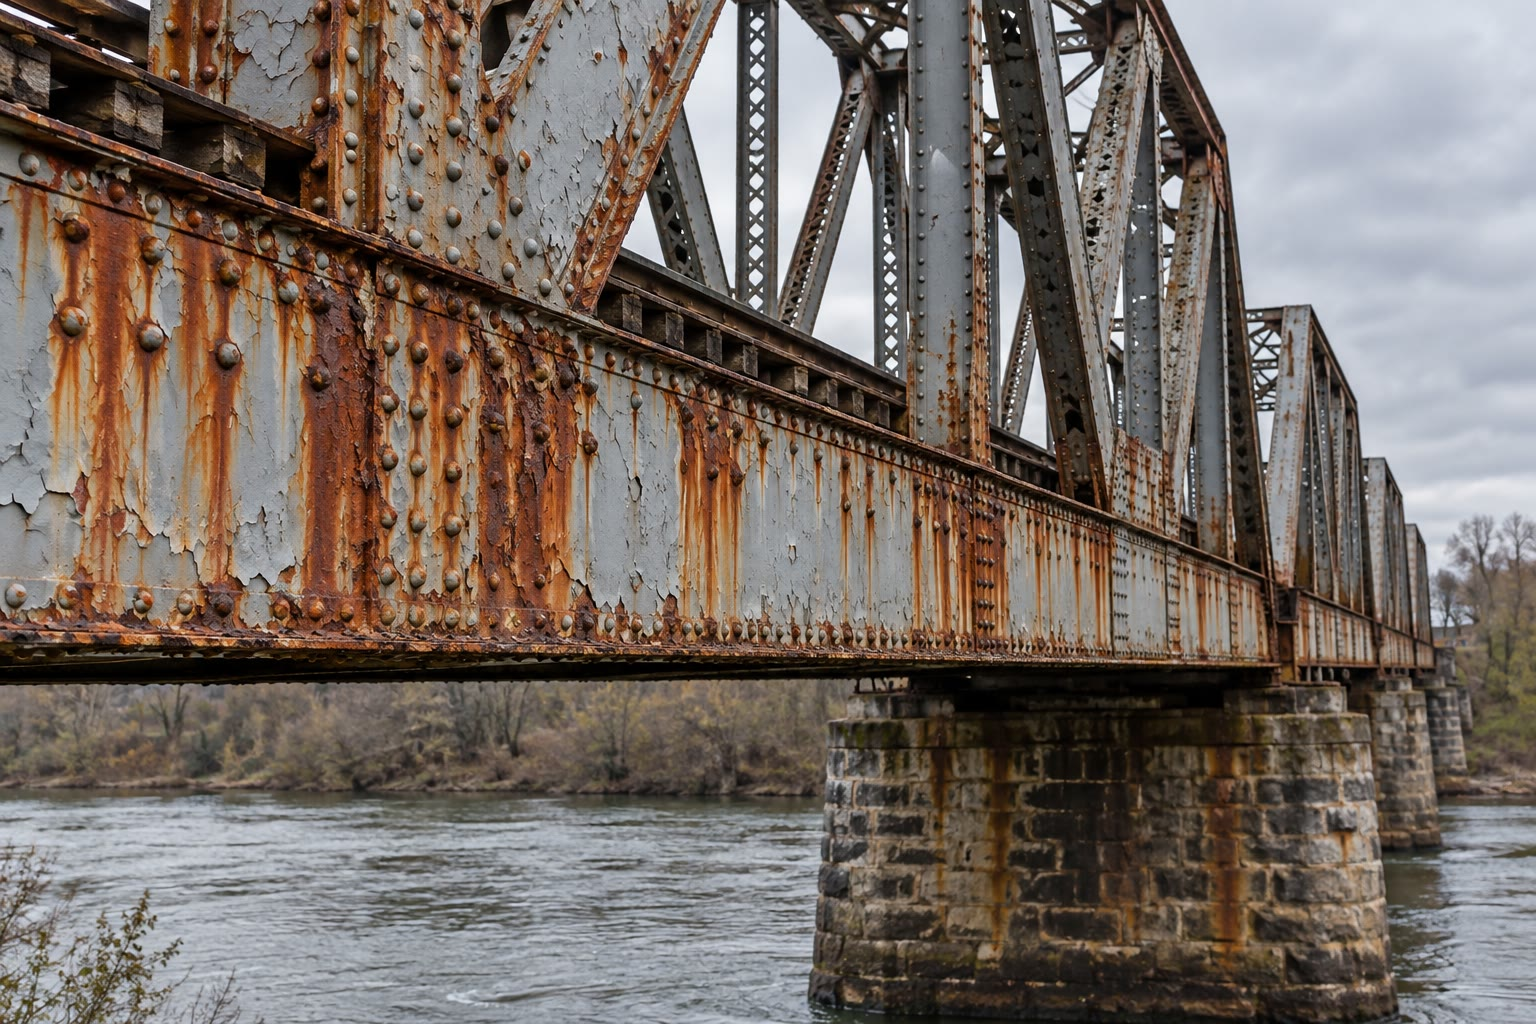
\includegraphics[width=0.62\linewidth]{images/book3/ai/b2-12-rusty-bridge.jpg}

{\small An old riveted railway bridge. Rust streaks run down from the rivets
and the joints, where water and oxygen stay longest and the paint fails
first.}
\end{omfigure}

\section{Wet corrosion as a short-circuited cell}

In water containing dissolved oxygen, iron is oxidised, \ce{Fe -> Fe^2+ + 2e-},
and the electrons are taken up on the same piece of metal by the reduction of
dioxygen, \ce{O2 + 2H2O + 4e- -> 4OH-} (in acid, also by \ce{2H+ + 2e- -> H2}). The
iron(II) ions and the hydroxide ions meet in the water, and further oxidation by
the air turns their precipitate into rust, a hydrated iron(III) oxide.

\begin{definition}[Uniform corrosion]\label{def:b2:corrosion:uniform}
\emph{Uniform corrosion}\index{uniform corrosion} is the corrosion of a metal
whose oxidation and the reduction of the oxidant take place at sites spread
evenly over its surface. The \emph{corrosion potential}\index{corrosion
potential} is the \omterm{def:b2:batteries-electrolysis:mixed-potential}{mixed potential} the metal then takes, and the
\emph{corrosion current}\index{corrosion current} the \omterm{def:b2:current-potential-curves:ie-curve}{anodic current} of the
metal's oxidation at that potential.
\end{definition}

\begin{omfigure}
\begin{tikzpicture}
\begin{axis}[omie, width=0.82\linewidth, height=5.6cm, xmin=-1.1, xmax=0.5,
  ymin=-1.6, ymax=1.6, xlabel={$E$}, ylabel={$i$}, clip=true, clip mode=individual,
  axis y line=left]
\addplot[omanodic] table[x=E, y=i] {figdata/out/bachelor-2-ie-curves-i-Fe.dat};
\addplot[omcathodic] table[x=E, y=i] {figdata/out/bachelor-2-ie-curves-i-O2.dat};
\addplot[omcathodic, densely dashed] table[x=E, y=i, y expr=-\thisrow{i}] {figdata/out/bachelor-2-ie-curves-i-O2.dat};
\draw[densely dotted] (axis cs:-0.394,-1.0) -- (axis cs:-0.394,1.0);
\fill (axis cs:-0.394,1.0) circle (1.4pt);
\node[font=\scriptsize, anchor=south east] at (axis cs:-0.40,1.02) {$i_{\text{corr}}$};
\node[font=\scriptsize, anchor=north west] at (axis cs:-0.39,-0.03) {$E_{\text{corr}}$};
\node[font=\scriptsize, omThm, anchor=west] at (axis cs:-0.35,1.4) {\ce{Fe} $\to$ \ce{Fe^2+}};
\node[font=\scriptsize, omDef, anchor=north west] at (axis cs:-0.75,-1.05) {\ce{O2} $\to$ \ce{OH-}, diffusion plateau};
\end{axis}
\end{tikzpicture}

{\small The Evans diagram of iron in aerated neutral water (model curves). The
cathodic curve of dioxygen is drawn also reflected upwards (dashed): the
\omterm{def:b2:corrosion:uniform}{corrosion potential} is where it meets the anodic curve of iron. As the
reduction of dioxygen has reached its diffusion plateau there, the \omterm{def:b2:corrosion:uniform}{corrosion
current} equals the \omterm{def:b2:current-potential-curves:limiting-current}{limiting current} of oxygen: stirring or aerating the water
makes iron corrode faster.}
\end{omfigure}

\begin{proposition}[Corrosion rate]\label{prop:b2:corrosion:rate}
A metal of molar mass $M$ and density $\rho$, oxidised with $n$ electrons per
atom under a \omterm{def:b2:corrosion:uniform}{corrosion current} density $j_{\text{corr}}$ (current per unit area),
loses per unit area and time the mass $j_{\text{corr}}M/(nF)$, that is a
thickness
\[
  \frac{de}{dt} = \frac{j_{\text{corr}}\,M}{nF\rho} .
\]
\end{proposition}

\begin{proof}
By \cref{prop:b2:current-potential-curves:current-rate}, the \omterm{def:b2:current-potential-curves:ie-curve}{anodic current}
density $j_{\text{corr}}$ oxidises $j_{\text{corr}}/(nF)$ moles of metal per unit area and
time; multiply by $M$ for the mass and divide by $\rho$ for the thickness.
\end{proof}

\begin{example}[Iron at \qty{10}{\micro A/cm^2}]\label{ex:b2:corrosion:rate}
With $j = \qty{0.10}{A/m^2}$, $M = \qty{55.845}{g/mol}$, $n = 2$, $\rho =
\qty{7.87}{g/cm^3}$: $de/dt = 0.10 \times 55.845/(2 \times 96\,485 \times 7.87
\times 10^6) = \qty{3.7e-12}{m/s}$, that is \qty{0.12}{mm} per year.
% ledger: aw:Fe, rho:Fe, const:F
\end{example}

\section{Differential corrosion}

\begin{definition}[Differential corrosion]\label{def:b2:corrosion:differential}
\emph{Differential corrosion}\index{differential corrosion} is a corrosion in
which the anodic and cathodic sites are separated, the metal being
oxidised preferentially at the anodic sites. It is \emph{galvanic
corrosion}\index{galvanic corrosion} when two different metals in electrical
contact share the same electrolyte, and \emph{differential
aeration}\index{differential aeration} when one metal is exposed to waters of
different oxygen contents.
\end{definition}

\begin{proposition}[Two metals in contact]\label{prop:b2:corrosion:galvanic}
When two metals in electrical contact dip into the same aerated water, they
take a single \omterm{def:b2:batteries-electrolysis:mixed-potential}{mixed potential}. The metal whose \omterm{def:b2:corrosion:uniform}{corrosion potential} is lower
becomes the anode and corrodes faster than alone; the other becomes a cathode,
on which dioxygen is reduced, and is protected.
\end{proposition}

\begin{proof}
Connected by a conductor of negligible resistance, the two metals are at the
same potential, where the sum of all \omterm{def:b2:current-potential-curves:ie-curve}{anodic currents} equals minus the sum of
all \omterm{def:b2:current-potential-curves:ie-curve}{cathodic currents}. The anodic curve of the less noble metal rises first;
at the common potential it carries nearly all of the \omterm{def:b2:current-potential-curves:ie-curve}{anodic current}, and the
oxygen is reduced on the whole wetted surface, including the nobler metal,
whose own \omterm{def:b2:current-potential-curves:ie-curve}{anodic current} is negligible there.
\end{proof}

\begin{omfigure}
\begin{tikzpicture}
\begin{axis}[omie, width=0.82\linewidth, height=5.6cm, xmin=-1.1, xmax=0.5,
  ymin=-2.4, ymax=2.4, xlabel={$E$}, ylabel={$i$}, clip=true, clip mode=individual,
  axis y line=left]
\addplot[omanodic] table[x=E, y=i] {figdata/out/bachelor-2-ie-curves-i-Fe.dat};
\addplot[omanodic, densely dashed] table[x=E, y=i] {figdata/out/bachelor-2-ie-curves-j-Zn.dat};
\addplot[omcathodic] table[x=E, y=i] {figdata/out/bachelor-2-ie-curves-i-O2.dat};
\addplot[omcathodic, densely dashed] table[x=E, y=i] {figdata/out/bachelor-2-ie-curves-j-O2Cu.dat};
\fill (axis cs:-0.394,1.0) circle (1.4pt);
\fill (axis cs:-0.794,1.0) circle (1.4pt);
\fill (axis cs:-0.366,2.0) circle (1.4pt);
\draw[densely dotted] (axis cs:-1.1,1.0) -- (axis cs:-0.394,1.0);
\draw[densely dotted] (axis cs:-1.1,2.0) -- (axis cs:-0.366,2.0);
\node[font=\scriptsize, anchor=south west] at (axis cs:-0.38,0.95) {iron alone};
\node[font=\scriptsize, anchor=west] at (axis cs:-0.35,2.0) {iron + copper};
\node[font=\scriptsize, anchor=south east] at (axis cs:-0.80,1.05) {iron + zinc};
\node[font=\scriptsize, omThm, anchor=north west] at (axis cs:-0.98,0.75) {zinc};
\node[font=\scriptsize, omThm, anchor=north west] at (axis cs:-0.55,0.75) {iron};
\node[font=\scriptsize, omDef, anchor=north east] at (axis cs:0.45,-2.05) {\ce{O2} on iron + copper};
\node[font=\scriptsize, omDef, anchor=north east] at (axis cs:0.45,-1.05) {\ce{O2} on iron};
\end{axis}
\end{tikzpicture}

{\small Iron coupled to other metals (model curves). With zinc, the common
potential falls to where zinc carries the \omterm{def:b2:current-potential-curves:ie-curve}{anodic current}: iron is protected,
zinc corrodes. With copper, the cathodic area for oxygen doubles: the
\omterm{def:b2:corrosion:uniform}{corrosion current} of iron doubles too.}
\end{omfigure}

\begin{proposition}[Differential aeration]\label{prop:b2:corrosion:aeration}
On a metal exposed to waters of different oxygen contents, the less aerated
zone is anodic and corrodes; the better aerated zone is cathodic.
\end{proposition}

\begin{proof}
Where the oxygen content is higher, the \ce{O2}/\ce{OH-} couple has a higher
Nernst potential and a larger \omterm{def:b2:current-potential-curves:limiting-current}{limiting current}: the cathodic curve lies higher
and reaches further. The metal, a single conductor, settles at one potential;
the large \omterm{def:b2:current-potential-curves:ie-curve}{cathodic current} available in the aerated zone must be balanced by an
\omterm{def:b2:current-potential-curves:ie-curve}{anodic current}, which flows where the metal can be oxidised with little
competition from oxygen reduction, the poorly aerated zone. Oxidation
concentrates there.
\end{proof}

\begin{omfigure}
\begin{tikzpicture}[font=\small, >={Stealth}]
  \fill[black!20] (-4.2,-0.7) rectangle (4.2,0);
  \node[font=\scriptsize] at (3.7,-0.35) {steel};
  \fill[omDef!15] (-3.4,0) .. controls (-2.9,2.2) and (2.9,2.2) .. (3.4,0) -- cycle;
  \draw[thick, omDef] (-3.4,0) .. controls (-2.9,2.2) and (2.9,2.2) .. (3.4,0);
  \fill[omProp!80] (-0.7,0) arc[start angle=180, end angle=360, x radius=0.7, y radius=0.22] -- cycle;
  \fill[brown!70!black] (-1.9,0.12) ellipse (0.45 and 0.11);
  \fill[brown!70!black] (1.9,0.12) ellipse (0.45 and 0.11);
  \node[font=\scriptsize, align=center] at (0,2.45) {\ce{O2} from the air};
  \draw[->, thick, omDef] (-1.0,2.25) -- (-2.6,0.35);
  \draw[->, thick, omDef] (1.0,2.25) -- (2.6,0.35);
  \node[font=\scriptsize, align=center, anchor=east] at (-4.1,1.3) {cathode\\ (rim)};
  \draw[->, thin] (-4.1,1.3) -- (-3.05,0.12);
  \node[font=\scriptsize, align=center, anchor=west] at (4.1,1.3) {rust ring};
  \draw[->, thin] (4.1,1.3) -- (2.3,0.2);
  \draw[->, omThm] (-0.4,-0.3) .. controls (-1.2,-0.5) and (-2.4,-0.5) .. (-3.0,-0.15);
  \draw[->, omThm] (0.4,-0.3) .. controls (1.2,-0.5) and (2.4,-0.5) .. (3.0,-0.15);
  \draw[->, thin] (0,-1.05) -- (0,-0.25);
  \node[font=\scriptsize, anchor=north] at (0,-1.05) {anode (centre): \ce{Fe -> Fe^2+ + 2e-}};
  \node[font=\scriptsize, omThm, anchor=north] at (0,-1.45) {electrons flow through the steel to the rim};
  \node[font=\scriptsize, anchor=north] at (0,-1.85) {cathode (rim): \ce{O2 + 2H2O + 4e- -> 4OH-}};
\end{tikzpicture}

{\small Evans's drop on steel, schematic. Oxygen dissolves at the surface and
reaches the metal mostly near the thin edge of the drop, which becomes the
cathode; the centre, starved of oxygen, is the anode and is pitted. The
iron(II) ions and the hydroxide ions meet in between, where the rust
precipitates as a ring.}
\end{omfigure}

The same mechanism attacks crevices, the parts of a structure under a deposit
or a gasket, and a steel pile in the sea just below the water line, where
the water is less aerated than at the surface.

\begin{method}[Diagnosing a corrosion]\label{met:b2:corrosion:diagnose}
\begin{enumerate}
  \item List the metals in contact and the electrolyte; check that they are
        electrically connected.
  \item For two metals, the one of lower \omterm{def:b2:corrosion:uniform}{corrosion potential} (usually the
        lower standard potential) is the anode.
  \item For one metal, find the less aerated zones (crevices, under deposits,
        the bottom of a drop): they are anodic.
  \item The rate is set by the cathodic reaction (oxygen supply, cathode area):
        a small anode on a large cathode corrodes fast.
\end{enumerate}
\end{method}

\section{Passivation}

\begin{definition}[Passivation]\label{def:b2:corrosion:passivation}
\emph{Passivation}\index{passivation} is the strong decrease of the corrosion
rate of a metal when it is covered by a thin, compact, adherent layer of its
oxide, the \emph{passive film}\index{passive film}, which separates it from the
solution. A metal in this state is said to be passive.
\end{definition}

\begin{proposition}[The passive plateau]\label{prop:b2:corrosion:passivity}
The anodic curve of a passivable metal rises from its \omterm{def:b2:corrosion:uniform}{corrosion potential},
reaches a peak, then falls to a small, nearly constant passive current over a
range of potentials, before rising again at high potentials (transpassive
region: oxidation of the film or of water). The passive state can break down
locally, for instance under chloride ions, giving pits.
\end{proposition}

\begin{proof}[Argument]
At low \omterm{def:b2:current-potential-curves:overpotential}{overpotentials} the bare metal dissolves faster and faster. Beyond a
threshold the oxide becomes stable at the surface (the \omterm{def:b2:corrosion:passivation}{passivation} domain of
the E--pH diagram) and forms a film through which ions move only slowly: the
current collapses to that small flux. At high potentials the film itself is
oxidised to soluble species, or water is oxidised on it. Chloride ions, small
and strongly complexing, can dissolve the film at weak points, where the bare
metal then corrodes as a small anode in front of a huge passive cathode. The
shape of the curve is a model here.
\end{proof}

\begin{omfigure}
\begin{tikzpicture}
\begin{axis}[omie, width=0.82\linewidth, height=5.4cm, xmin=-0.7, xmax=1.5,
  ymin=-0.1, ymax=1.3, xlabel={$E$}, ylabel={$i$}, clip=true, clip mode=individual,
  axis y line=left]
\addplot[omanodic] table[x=E, y=i] {figdata/out/bachelor-2-ie-curves-k.dat};
\node[font=\scriptsize, anchor=south] at (axis cs:-0.33,1.0) {active};
\node[font=\scriptsize, anchor=south] at (axis cs:0.5,0.06) {passive plateau};
\node[font=\scriptsize, anchor=east] at (axis cs:1.25,0.9) {transpassive};
\draw[<-, thin] (axis cs:-0.2,0.55) -- (axis cs:0.15,0.7) node[right, font=\scriptsize] {film forms};
\end{axis}
\end{tikzpicture}

{\small Anodic curve of a passivable metal (model). The current, large while
the bare metal dissolves, collapses when the \omterm{def:b2:corrosion:passivation}{passive film} forms, and stays
small over a wide range of potentials before the transpassive rise.}
\end{omfigure}

Stainless steels hold enough chromium to form a passive chromium oxide film
that heals itself in air; aluminium is protected by its alumina film, which
makes a metal far below hydrogen in the series usable for window frames and
drinks cans. Copper turns green in the open air, the patina being a layer of
basic copper salts that slows further attack.

\begin{omfigure}

\includegraphics[width=0.32\linewidth]{images/book3/liberty.jpg}

{\small A copper statue more than a century old: its skin of thin copper sheet
has turned green, covered by a patina of basic copper salts that protects the
metal beneath. (Photograph: Elcobbola, public domain, Wikimedia Commons.)}
\end{omfigure}

\section{Protection}

Corrosion is fought by separating the metal from water and oxygen (paint,
plastic, enamel, or a layer of another metal), by changing the medium
(removing oxygen, adding inhibitors that adsorb on the metal), or by shifting the
potential of the metal into its domain of immunity.

\begin{definition}[Cathodic protection]\label{def:b2:corrosion:protection}
\emph{Cathodic protection}\index{cathodic protection} lowers the potential of a
metal structure until its oxidation stops, by making it the cathode of a cell.
The cell can be formed with a \emph{sacrificial anode}\index{sacrificial
anode}, a less noble metal (zinc, magnesium, aluminium alloys) connected to the
structure and consumed in its place, or driven by a generator, in
\emph{impressed-current protection}\index{impressed-current protection}, the
anode being then an inert electrode buried nearby.
\end{definition}

\begin{proposition}[Lifetime of a sacrificial anode]\label{prop:b2:corrosion:anode-life}
A \omterm{def:b2:corrosion:protection}{sacrificial anode} of mass $m$ and molar mass $M$, oxidised with $n$ electrons
and an efficiency $\eta$ (the fraction of the metal that produces useful
current, the rest corroding by itself), delivers a current $I$ for a time
\[
  t = \frac{\eta\,m\,nF}{M I} .
\]
\end{proposition}

\begin{proof}
The useful charge is $\eta\,(m/M)\,nF$; divide by the current.
\end{proof}

\begin{omfigure}
\begin{tikzpicture}[font=\small, >={Stealth}]
  \fill[brown!20] (-4.2,-2.4) rectangle (4.2,0);
  \draw[thick] (-4.2,0) -- (4.2,0);
  \node[font=\scriptsize, anchor=south west] at (-4.2,0) {ground};
  \fill[black!40] (-3.5,-1.6) rectangle (3.5,-1.2);
  \node[font=\scriptsize, white] at (0,-1.4) {steel pipe (cathode)};
  % sacrificial anode
  \fill[black!65] (-3.2,-2.3) rectangle (-2.2,-1.95);
  \node[font=\scriptsize, anchor=north] at (-2.7,-2.3) {Mg anode};
  \draw[thick] (-2.7,-1.95) -- (-2.7,-1.6);
  \draw[->, omProp, thick] (-2.2,-2.12) -- (-1.4,-1.7);
  \node[font=\scriptsize, omProp, anchor=west] at (-1.9,-2.2) {current in the soil};
  % impressed current
  \draw[thick, rounded corners] (1.8,0.4) rectangle (3.2,1.2);
  \node[font=\scriptsize] at (2.5,0.8) {rectifier};
  \fill[black!65] (3.4,-2.3) rectangle (3.9,-1.8);
  \node[font=\scriptsize, anchor=north] at (3.65,-2.3) {inert anode};
  \draw[thick] (3.2,0.8) -- (3.65,0.8) -- (3.65,-1.8);
  \draw[thick] (1.8,0.8) -- (1.2,0.8) -- (1.2,-1.2);
  \node[font=\scriptsize, anchor=south] at (3.65,0.85) {$+$};
  \node[font=\scriptsize, anchor=south] at (1.2,0.85) {$-$};
  \node[font=\scriptsize, align=center] at (-2.7,0.8) {sacrificial anode};
  \node[font=\scriptsize, align=center] at (2.5,1.55) {impressed current};
\end{tikzpicture}

{\small \omterm{def:b2:corrosion:protection}{Cathodic protection} of a buried pipe, schematic. Left: a magnesium
anode, wired to the pipe, corrodes in its place. Right: a rectifier drives a
current from an inert anode through the soil into the pipe.}
\end{omfigure}

\begin{omfigure}
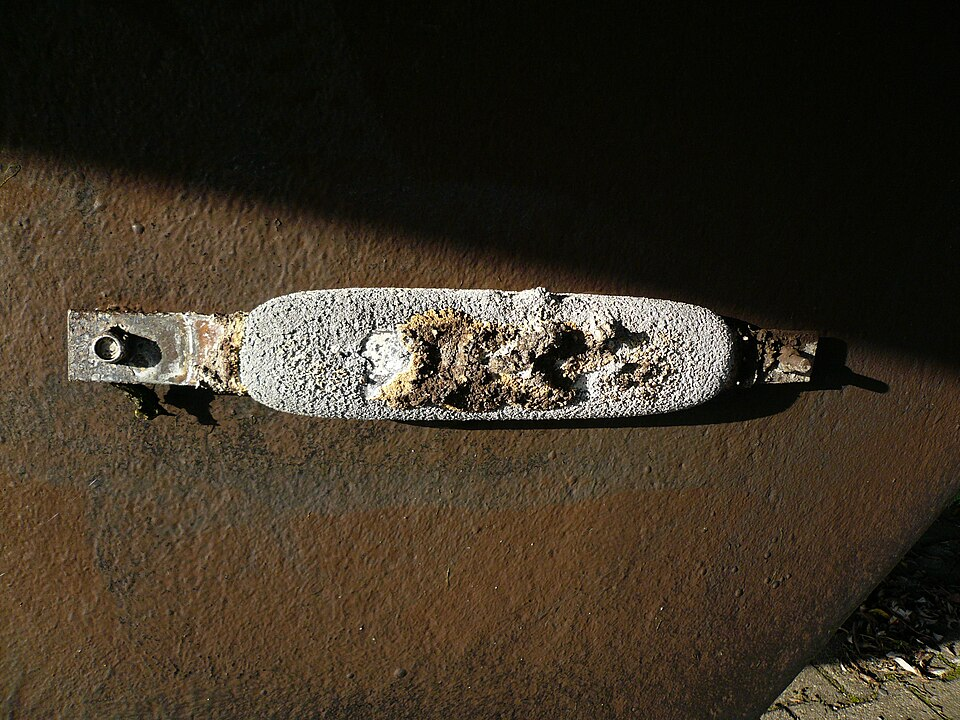
\includegraphics[width=0.5\linewidth]{images/book3/sacrificial-anode.jpg}

{\small A zinc \omterm{def:b2:corrosion:protection}{sacrificial anode} bolted to the steel hull of a boat, after a
season in the water: the zinc is eaten away, the steel around it is intact.
(Photograph: Zwergelstern, CC BY-SA 3.0, Wikimedia Commons.)}
\end{omfigure}

\begin{omfigure}
\begin{tikzpicture}[font=\small, >={Stealth}, scale=1.35]
  \begin{scope}
    \fill[black!25] (0,0) rectangle (4,0.6);
    \fill[gray!55] (0,0.6) rectangle (1.7,0.8); \fill[gray!55] (2.3,0.6) rectangle (4,0.8);
    \fill[omDef!15] (0.8,0.8) .. controls (1.3,1.3) and (2.7,1.3) .. (3.2,0.8) -- (2.3,0.8) -- (2.3,0.6) -- (1.7,0.6) -- (1.7,0.8) -- cycle;
    \node[font=\scriptsize] at (2,-0.3) {galvanised steel (zinc layer)};
    \node[font=\scriptsize, align=center] at (2,1.6) {zinc corrodes,\\ steel protected};
    \draw[->, omThm] (1.4,0.85) -- (1.8,0.65);
  \end{scope}
  \begin{scope}[xshift=5.5cm]
    \fill[black!25] (0,0) rectangle (4,0.6);
    \fill[gray!25] (0,0.6) rectangle (1.7,0.8); \fill[gray!25] (2.3,0.6) rectangle (4,0.8);
    \fill[omDef!15] (0.8,0.8) .. controls (1.3,1.3) and (2.7,1.3) .. (3.2,0.8) -- (2.3,0.8) -- (2.3,0.6) -- (1.7,0.6) -- (1.7,0.8) -- cycle;
    \fill[omProp] (1.75,0.6) rectangle (2.25,0.45);
    \node[font=\scriptsize] at (2,-0.3) {tinned steel (tin layer)};
    \node[font=\scriptsize, align=center] at (2,1.6) {steel corrodes in the scratch,\\ fast (small anode)};
  \end{scope}
\end{tikzpicture}

{\small A scratch through a metal coating, schematic. Zinc, less noble than
iron, becomes the anode and protects the exposed steel, whatever the size of
the scratch. Tin, nobler than iron, becomes a large cathode around a small
steel anode, which corrodes faster than bare steel would.}
\end{omfigure}

\begin{method}[Choosing a protection]\label{met:b2:corrosion:choose-protection}
\begin{enumerate}
  \item Avoid galvanic couples: insulate dissimilar metals, or make the less
        noble one the larger.
  \item Coat: a barrier coat (paint, tin) only protects while intact; a
        sacrificial coat (zinc) protects even when scratched.
  \item For a structure in soil or sea water, add \omterm{def:b2:corrosion:protection}{cathodic protection}:
        \omterm{def:b2:corrosion:protection}{sacrificial anodes} for small currents or conductive water,
        impressed current for long structures or resistive soils.
  \item Do not over-protect: too low a potential reduces water to hydrogen at
        the structure, which lifts coatings and can embrittle high-strength
        steels.
\end{enumerate}
\end{method}

\section{Exercises}

\begin{exercise}[$\star$]\label{exo:b2:corrosion:1}
Zinc corrodes uniformly under a current density of \qty{2.0}{\micro A/cm^2}.
Compute its loss of thickness per year ($\rho = \qty{7.13}{g/cm^3}$).
\end{exercise}

\begin{exercise}[$\star$]\label{exo:b2:corrosion:2}
Steel bolts hold copper sheets on a roof. Which metal corrodes? Same question
for zinc nails in steel sheets.
\end{exercise}

\begin{exercise}[$\star$]\label{exo:b2:corrosion:3}
Two steel plates are held together by a bolt and left in sea water. Where does
the corrosion concentrate, and why?
\end{exercise}

\begin{exercise}[$\star$]\label{exo:b2:corrosion:4}
A galvanised bucket and a tin can are both scratched down to the steel. Which
one rusts at the scratch?
\end{exercise}

\begin{exercise}[$\star\star$]\label{exo:b2:corrosion:5}
On the Evans diagram of iron in aerated water, explain what happens to the
\omterm{def:b2:corrosion:uniform}{corrosion potential} and current when the water is stirred, then when it is
freed from oxygen.
\end{exercise}

\begin{exercise}[$\star\star$]\label{exo:b2:corrosion:6}
A zinc anode of \qty{5.0}{kg} protects a boat hull with a current of
\qty{0.10}{A}, with an efficiency of 90~\% (exercise data). How long does it
last?
\end{exercise}

\begin{exercise}[$\star\star$]\label{exo:b2:corrosion:7}
Compute the charge, in ampere-hours per kilogram, delivered by zinc, magnesium
and aluminium anodes at 100~\% efficiency, and the standard potentials of
their couples from $\Delta_f G^\circ$ (\ce{Zn^2+} $-147.06$, \ce{Mg^2+} $-454.8$,
\ce{Al^3+} $-485$ \unit{kJ/mol}). Why is magnesium preferred in dry soils?
\end{exercise}

\begin{exercise}[$\star\star$]\label{exo:b2:corrosion:8}
A buried pipe needs \qty{2.0}{A} of protection current. The ground bed of the
inert anode has a resistance of \qty{4.0}{\ohm} to the soil and the cell needs a
further \qty{1.5}{V} (exercise data). Compute the voltage of the rectifier and the
electrical energy per year.
\end{exercise}

\begin{exercise}[$\star\star$]\label{exo:b2:corrosion:9}
A steel pile stands in the sea. Explain why it corrodes most a little below
the water line, and not at the water line itself.
\end{exercise}

\begin{exercise}[$\star\star\star$]\label{exo:b2:corrosion:10}
Explain, with the passive curve, why stainless steel resists aerated water but
may pit in sea water, and why a pit, once started, grows deeper rather than
wider.
\end{exercise}

\begin{exercise}[$\star\star\star$]\label{exo:b2:corrosion:11}
A copper fitting is screwed on a steel pipe carrying aerated water. The oxygen
\omterm{def:b2:current-potential-curves:limiting-current}{limiting current} density is \qty{5}{\micro A/cm^2} on every wetted surface; the
copper offers \qty{20}{cm^2} and the steel near the joint \qty{2}{cm^2}
(exercise data). Estimate the \omterm{def:b2:corrosion:uniform}{corrosion current} of the steel and its loss of
thickness per year near the joint.
\end{exercise}

\begin{exercise}[$\star\star\star$]\label{exo:b2:corrosion:12}
Using the E--pH diagram of iron and the curves of water, explain why the
potential of a protected steel structure should be held below about
\qty{-0.6}{V} but not far below \qty{-1}{V} in neutral water.
\end{exercise}

\section{Problem: Protecting a Pipeline}

\begin{problem}[{Weekend problem --- the corrosion of a bare steel pipe in wet
soil, the choice of a sacrificial metal, the magnesium needed for twenty years,
and the impressed-current alternative}]
\label{pb:b2:corrosion:1}
A steel pipeline \qty{10.0}{km} long and \qty{0.30}{m} in diameter is buried in
wet soil. Data: iron $M = \qty{55.845}{g/mol}$, $\rho = \qty{7.87}{g/cm^3}$;
magnesium $M = \qty{24.305}{g/mol}$; $\Delta_f G^\circ$ (\unit{kJ/mol}): \ce{Fe^2+}
$-78.90$, \ce{Zn^2+} $-147.06$, \ce{Mg^2+} $-454.8$, \ce{Al^3+} $-485$. Exercise
data: \omterm{def:b2:corrosion:uniform}{corrosion current} density of bare steel in this soil \qty{10}{\micro
A/cm^2}; design current density for the protection of bare steel
\qty{20}{mA/m^2}; the coating leaves 1.0~\% of the surface bare; magnesium anodes
of \qty{15}{kg}, efficiency 50~\%; ground-bed resistance for the impressed current
\qty{5.0}{\ohm}.
% ledger: aw:Fe, rho:Fe, aw:Mg, dfg:Fe2+_ao, dfg:Zn2+_ao, dfg:Mg2+_ao, dfg:Al3+_ao, const:F

\medskip
\noindent\textbf{Part I --- The bare pipe.}
\begin{enumerate}
  \item Write the anodic and cathodic reactions on the pipe.
  \item Why is the \omterm{def:b2:corrosion:uniform}{corrosion current} set by the supply of oxygen?
  \item Compute the mass of iron lost per square metre and per year.
  \item Compute the loss of wall thickness per year.
  \item How long would the bare pipe take to lose half of an \qty{8}{mm} wall?
  \item Why does the real pipe fail sooner, at a few points?
\end{enumerate}

\medskip
\noindent\textbf{Part II --- The anode metal.}
\begin{enumerate}[resume]
  \item Compute the standard potentials of the couples of iron, zinc, magnesium
        and aluminium.
  \item Which metals can protect iron as \omterm{def:b2:corrosion:protection}{sacrificial anodes}?
  \item Why is aluminium little used in soils?
  \item Why is magnesium preferred to zinc in a soil of high resistivity?
  \item Compute the mass of magnesium consumed per ampere and per year.
\end{enumerate}

\medskip
\noindent\textbf{Part III --- Design.}
\begin{enumerate}[resume]
  \item Compute the outer surface of the pipe.
  \item Compute the bare surface left by the coating.
  \item Compute the protection current.
  \item Compute the charge needed for twenty years.
  \item Compute the mass of magnesium needed.
  \item How many anodes are needed?
  \item Why are they distributed along the pipe rather than buried at one
        point?
\end{enumerate}

\medskip
\noindent\textbf{Part IV --- Impressed current.}
\begin{enumerate}[resume]
  \item Describe the impressed-current alternative.
  \item Estimate the voltage of the rectifier from the ground-bed resistance,
        adding \qty{1.5}{V} for the electrodes.
  \item Compute the electrical energy used per year.
  \item What goes wrong if the pipe is over-protected?
  \item Below which potential is iron immune in neutral water, taking an
        iron(II) concentration of \qty{1e-6}{mol/L}?
  \item State the mass of magnesium anodes needed for twenty years.
\end{enumerate}
\end{problem}
